
\begin{figure*}[ht]
\begin{subfigure}[t]{.33\textwidth}
  \centering
   \captionsetup{width=.9\linewidth}
    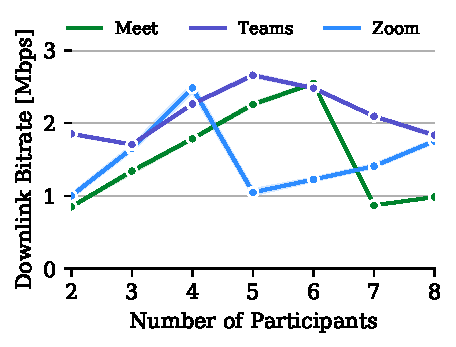
\includegraphics[width=1\textwidth,keepaspectratio]{../figures/modality/speaker_recv.pdf}
    \caption{Downlink traffic of client whose video is viewed in gallery mode}
    \label{fig:gallery-recv}
\end{subfigure}
\hfill
\begin{subfigure}[t]{.33\textwidth}
  \centering
   \captionsetup{width=.9\linewidth}
    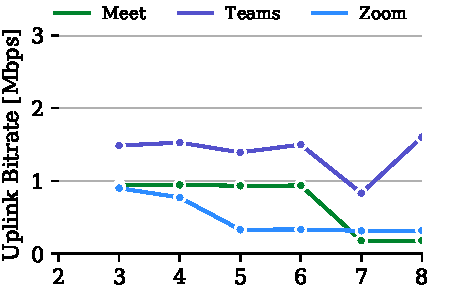
\includegraphics[width=1\textwidth,keepaspectratio]{../figures/modality/gallery_send.pdf}
    \caption{Uplink traffic of client whose video is viewed in gallery mode}
    \label{fig:gallery-send}
\end{subfigure}
\hfill
\begin{subfigure}[t]{.33\textwidth}
  \centering
   \captionsetup{width=.9\linewidth}
    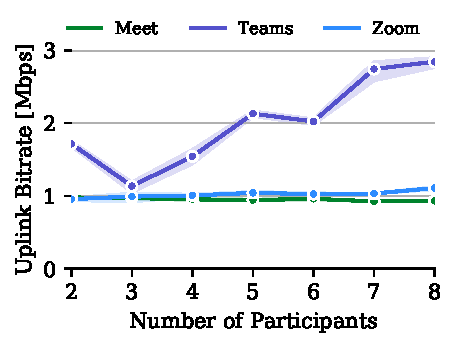
\includegraphics[width=1\textwidth,keepaspectratio]{../figures/modality/speaker_send.pdf}
    \caption{Uplink traffic of client whose video is pinned by all other participants}
    \label{fig:speaker-send}
\end{subfigure}
\caption{Network utilization in different viewing modalities}
\label{fig:viewing-mode}
\end{figure*}

\section{Call Modalities}\label{sec:usage_modality}





%Until now, we have focused on the performance and network utilization of 2-person calls.

Up to this point we have only considered 2-person calls. However, with people using VCAs for work and school, it is more common to have large number of participants. We now look at network utilization under two prominent call modalities: the number of participants in a call and the viewing mode. We consider two viewing modes that are common across all three VCAs: \textit{speaker} mode wherein a specific user's video is pinned on the call and \textit{gallery} mode, in which all participants' video are shown on the screen. Our goal is to understand the impact of these call modalities on VCA's network utilization. Each experiment consists of a 2-minute call with $n$ users and specific viewing mode. We vary the number of clients in the call: \{2, 3, .., 8\} and viewing mode: \{gallery, speaker\}. Each modality is repeated 5 times and we log the network utilization of Client 1 (\textbf{C1}) in each call. 


\subsection{Number of users}
We fix the viewing mode to \textit{gallery} which is the default viewing mode in all the VCAs. Figure~\ref{fig:gallery-recv} and~
\ref{fig:gallery-send} show the average downlink and uplink network utilization respectively, as the number of participants vary in a call. Interestingly, both downlink and uplink utilization can reduce as the number of participants increase in a call for \meet and \zoom. For \zoom, the uplink utilization drops from 0.8 Mbps to 0.4 Mbps as number of participants change from 4 to 5. For \meet, the reduction happens at n = 7 from 1 Mbps to  0.2 Mbps. We observe that both \meet and \zoom have tiled-screen display with each user displayed in a separate tile. Clearly, as the number of users increases, the tile size shrinks to accommodate all the users on the fixed size screen. As a result, the sender sees this as an opportunity to reduce the its sent video resolution, leading to reduction in uplink utilization.


We see a similar drop in the downlink utilization at 5 and 7 participants for \zoom and \meet, respectively (Figure~\ref{fig:gallery-recv}). However, there are also notable differences when compared to the uplink utilization. For instance, the downlink utilization for Google Meet increases from 1.25 Mbps to 2.5 Mbps when number of participants change from 3 to 6, while the uplink utilization stays mostly constant. The trend is similar for \zoom as number of participants become more than 5. The difference is because downlink utilization also depends on number of video streams in addition to the data rate of each stream. Thus, if the per-user resolution remains the same, the downlink utilization would increase as the number of participants increases in a call. 

Interestingly, we don't observe any such trend in \teams. The uplink utilization remains almost constant as the number of participants change. The downlink utilization increases until 5 participants and drops as more participants join the call. We observe that \teams has a fixed 4-tile layout on Linux. It thus displays only a subset of participants if the total participants are more than 4. This can explain why the sending rate does not change as the picture size may not change significantly with more users. It is, however, not clear why the downlink utilization drops after 5 participants. We plan to dig deeper into this in the future work by also inspecting the network traffic on the other clients. 
% As a result, the sender's video resolution decreases leading to reduction in the uplink utilization. The downlink utilization 
 % We observe that Teams is also exhibiting a downward trend at 8 participants. It should be noted that while the size of the tile shrinks with more participants in Meet and Zoom,  This feature explains why we do not see the same downward trend in Teams.
 



\subsection{Viewing mode}
We find that viewing a user's video in speaker mode leads to greater uplink consumption on the user's network as compared to gallery mode for all three VCAs. Putting C1 on the speaker mode enlarges its tile size on other users' screen. The sender does not reduce the video resolution to provide a high video quality, thus leading to increase in uplink utilization compared to when C1 was not pinned by other users. \zoom and \meet consistently send at 1 Mbps when all clients pin C1's video, regardless of the number of participants. Note that, only one client needed to put C1 on speaker for this behavior. Each client can decide to pin any client independently of others.

We find that the behavior of \teams differs here as well from \meet and \zoom. C1's uplink utilization continues to increase from 1.25 Mbps with 3 participants to 2.9 Mbps participants when it is put on speaker mode. We checked if the increase could be attributed to \teams communicating with multiple destinations (e.g., with each user separately). However, we observe that all of the traffic was directed to a single server. It is not clear what contributes to the increase in traffic for \teams but this clearly leads to inefficient network utilization, especially when compared to \zoom and \meet. 

\begin{mdframed}[roundcorner=5pt, backgroundcolor=black!10]
\paragraph{Takeaways}: Each participant's video layout impacts client's network utilization. Both uplink and dowlink utilization can decrease with more participants depending on how the VCA displays participant video. Additionally, when other participants pin the client's video (speaker mode), the client's uplink utilization can increase. 
\end{mdframed}

